\documentclass{article}


% if you need to pass options to natbib, use, e.g.:
%     \PassOptionsToPackage{numbers, compress}{natbib}
% before loading neurips_2023


% ready for submission
\usepackage[final]{neurips_2023}


% to compile a preprint version, e.g., for submission to arXiv, add add the
% [preprint] option:
%     \usepackage[preprint]{neurips_2023}


% to compile a camera-ready version, add the [final] option, e.g.:
%     \usepackage[final]{neurips_2023}


% to avoid loading the natbib package, add option nonatbib:
%    \usepackage[nonatbib]{neurips_2023}


\usepackage[utf8]{inputenc} % allow utf-8 input
\usepackage[T1]{fontenc}    % use 8-bit T1 fonts
\usepackage{hyperref}       % hyperlinks
\usepackage{url}            % simple URL typesetting
\usepackage{booktabs}       % professional-quality tables
\usepackage{amsfonts}       % blackboard math symbols
\usepackage{nicefrac}       % compact symbols for 1/2, etc.
\usepackage{microtype}      % microtypography
\usepackage{xcolor}         % colors


% OWN PACKAGES AND SETTINGS

\usepackage{amsmath,amsthm,amssymb} % for the common "math symbols"
\usepackage{mathrsfs}
\usepackage{mathtools}
\usepackage{caption}
\usepackage{subcaption}
\usepackage{wrapfig}



% STRUCTURE
\newtheorem{theorem}{Theorem}
\newtheorem{lemma}[theorem]{Lemma}


% CUSTOM COMMANDS
\newcommand{\set}[1]{\left\{#1\right\}}
\newcommand{\multiset}[1]{\left\{\!\!\left\{#1\right\}\!\!\right\}}
\newcommand{\iter}[1]{^{(#1)}}
\newcommand{\wl}{\texttt{wl}}
\newcommand{\wledge}{\texttt{wl-ed}}
\newcommand{\lwl}{\texttt{lwl}}
\newcommand{\norm}[1]{\left\lVert#1\right\rVert}
\newcommand{\upd}{\texttt{UPD}}
\newcommand{\agg}{\texttt{AGG}}
\newcommand{\dec}{\xi}
\newcommand{\initdec}{\xi}
\newcommand{\hash}{\tau}
\newcommand{\nbh}{\mathcal{N}}
\newcommand{\bs}[1]{\boldsymbol{#1}}
\newcommand{\feat}{\bs{h}}

\newcommand{\mca}{\mathcal{A}}
\newcommand{\mcb}{\mathcal{B}}
\newcommand{\mcc}{\mathcal{C}}
\newcommand{\mcd}{\mathcal{D}}
\newcommand{\mce}{\mathcal{E}}
\newcommand{\mck}{\mathcal{K}}
\newcommand{\mcl}{\mathcal{L}}
\newcommand{\mcm}{\mathcal{M}}
\newcommand{\mcn}{\mathcal{N}}
\newcommand{\mcq}{\mathcal{Q}}
\newcommand{\mcs}{\mathcal{S}}
\newcommand{\mct}{\mathcal{T}}
\newcommand{\mcv}{\mathcal{V}}

\newcommand{\mbb}{\mathbb{B}}
\newcommand{\mbe}{\mathbb{E}}
\newcommand{\mbi}{\mathbb{I}}
\newcommand{\mbk}{\mathbb{K}}
\newcommand{\mbn}{\mathbb{N}}
\newcommand{\mbr}{\mathbb{R}}
\newcommand{\mbz}{\mathbb{Z}}

\newcommand{\msk}{\mathscr{K}}
\newcommand{\msl}{\mathscr{L}}
\newcommand{\msw}{\mathscr{W}}



\title{Expressiveness of Line Graph Neural Networks}
\author{%
    1083152
}


\begin{document}
\maketitle


\begin{abstract}

\end{abstract}


\section{Introduction}
% Start with graph structured data - ubiquitous in real-world applications, such as social networks, biological networks, recommendation systems, material science, traffic networks, etc.
Graphs are a natural way to structure data in many application domains, such as social networks, biological networks, recommendation systems, materials science, traffic networks, etc.
% Graph neural networks
Following the many successes of deep learning, graph machine learning has emerged as a powerful tool to learn from graph-structured data. There are various tasks that are of interest, including classification, link prediction and property prediction, but also graph generation and community detection.

% Line graph neural networks - especially natural for the task of link prediction
Recently, several works have investigated the use of line graphs in graph machine learning \cite{cai2021line,choudhary2021atomistic}. Line graphs offer a dual perspective on the original graph, where nodes in the line graph correspond to edges in the original graph. This perspective is especially natural for the task of link prediction, as it converts a classification task on pairs of nodes to the simpler and better studied task of node classification.

% Expressive power
The theoretical understanding of these models, however, is still in its infancy.
% State research question
In this work we therefore aim to characterize the expressive power of graph neural networks operating on line graphs. We will specifically focus on message-passing neural networks operating on line graphs, henceforth called Line Graph MPNNs (LG-MPNNs).

% Summarize contributions
Our contributions can be summarized as follows:
\begin{itemize}
    \item We introduce two new variations of the Weisfeiler-Leman test tailored to edge colourings, which we call the \emph{Line Weisfeiler-Leman Test} (LWL) and the \emph{Weisfeiler-Leman Test with Edge Decoding} (WL-ED).
    \item We prove both an upper and a lower bound on the expressivity of LG-MPNNs: they are at most as expressive as LWL and there exist Line Graph MPNNs that are equally expressive as LWL.
    \item We relate LWL and WL-ED to each other and to the standard Weisfeiler-Leman test for node colouring. We prove that LWL is strictly less expressive than WL-ED and that WL-ED is equally expressive as the standard Weisfeiler-Leman test.
\end{itemize}


\section{Related Work}

\paragraph{Graph Neural Networks}
% focus on isomorphism and permutation invariance/equivariance
Graph neural networks (GNNs) are a class of neural networks specifically designed to operate on graph-structured data \cite{scarselli2008graph}. One of the key challenges in designing GNNs is handling the inherent permutation invariance of graphs: since a graph with permuted node labels is still the same graph, the output of the network should not be affected by the ordering of the node labels either.
% message passing
The most commonly used class of GNNs are message passing neural networks (MPNNs) \cite{gilmer2017neural}, which iteratively update node features by aggregating information from neighbouring nodes. Many GNN architectures fall under this framework, including the Basic GNN model \cite{hamilton2020graph}, GAT \cite{velickovic2017graph}, and Graph Isomorphism Networks \cite{xu2018powerful}.


\paragraph{Expressiveness}
% start with expressive power of neural networks in general
% then move to graph neural networks
% state both graph/node distinguishability and function approximation as ways to characterize expressiveness
The expressive power of a parametrized model refers to the range of functions and patterns that it can represent. 
% TODO: something about general neural networks?
In the context of graph neural networks, there are various ways to characterize expressiveness. The most common one is the ability to distinguish non-isomorphic graphs, but the to function approximation \cite{maron2019universality}, substructure counting \cite{chen2020can}, spectral decomposition \cite{balcilar2020analyzing} and logical representation \cite{barcelo2020logical} are other viable criterions. Interestingly, \cite{chen2019equivalence} showed a theoretical equivalence between the expressiveness in terms of graph distinguishability and function approximation on graphs.

In this work, we mainly focus on expressiveness in terms of distinguishing non-isomorphic graphs.
The usual way to quantify this expressiveness is through a comparison with various forms of the Weisfeiler-Leman (WL) test \cite{weisfeiler1968reduction}. Importantly, MPNNs are known to be at most as expressive as the standard WL-test \cite{morris2019weisfeiler}, while \cite{xu2018powerful} constructed a class of GNNs that is equally expressive as WL. Other works have introduced other variations of the WL-test, such as the $k$-WL hierarchy \cite{morris2019weisfeiler} and the Relational Asymmetric Local 2-WL \cite{huang2024theory}.
Our work aligns with this line of research by introducing two new variations of the WL-test tailored to edge colourings, by characterizing the expressive power of LG-MPNNs in terms of these tests, and by placing these tests in the $k$-WL hierarchy.



\paragraph{Line Graph Neural Networks}
Most methods that use line graphs in graph machine learning do so in combination with the original graph \cite{choudhary2021atomistic,chen2017supervised,jiang2019censnet,zhang2023line}. For example, \cite{zhang2023line} runs GNNs on the original graph and the line graph in parallel, and then maximizes the mutual information between the two outputs.
Further, it should be noted that most methods that compute edge attributes, e.g. 
Generalized Message Passing \cite{battaglia2018relational}, could also be regarded as operating on the line graph.
A few approaches have also been proposed that operate only on the line graph, such as LGLP \cite{cai2021line} and INDIGO \cite{liu2021indigo}.
We limit the scope of this study to these approaches, as their analysis will also be of benefit to the compound methods. To the best of our knowledge, no work has yet been done on the theoretical analysis of these models.



\section{Background}    \label{sec:background}
% Summary of notations?

\paragraph{Graphs}
% + Line graphs
% + Graph Colourings
% + Node colourings of line graphs
A \emph{graph} is a tuple $G=(V,E,c)$ where $V$ is a set of nodes, $E\subseteq V\times V$ is a set of edges, and $c: V\rightarrow\mcc$ is a node colouring. In this work, we consider undirected, simple graphs.
The reason for limiting ourselves to node-coloured graphs despite the focus on models that compute edge features is to fit in the existing literature on the Weisfeiler-Leman test and allow for a direct comparison. We will often write $u\in G$ as a shorthand for $u\in V(G)$.
The \emph{neighbourhood} of a node $u\in V$ is $\nbh(u) = \set{v\in V \mid (u,v)\in E}$. The \emph{disjoint union} $G_1 \sqcup G_2$ of two graphs is the graph with node set $V(G_1) \sqcup V(G_2)$ and edge set $E(G_1) \sqcup E(G_2)$ that retains the colouring of the nodes.
The \emph{line graph} $L(G)$ of $G$ is a graph whose nodes correspond to the edges of $G$, where we denote the node in $L(G)$ corresponding to the edge $(u,v)\in E(G)$ by $uv$. Two nodes in $L(G)$ are connected if and only if the corresponding edges in $G$ share a node. Finally, the node colouring of $L(G)$ is $c: V(L(G)) \rightarrow \mcc: uv \mapsto \initdec(\set{c(u),c(v)})$, where $\initdec$ is an injective function from $\mcc^2$ to $\mcc$, i.e. two nodes in $L(G)$ get the same label iff the endpoints of their corresponding edges had the same set of labels in $G$. This is a variation of the atomic type defined in \cite{morris2019weisfeiler} tailored to undirected edges.

\paragraph{Message Passing Neural Networks}
% Framework with update/aggregate functions
A Message Passing Neural Network (MPNN) \cite{gilmer2017neural} is a framework for learning on graph-structured data that works by iteratively aggregating and updating node features. The feature of node $u$ in iteration $t$ is denoted as $\feat_u\iter{t}$. It starts with $\feat_u\iter{0} = c(u)$ and then iteratively updates the features of all nodes $u\in G$ as follows:
\begin{equation}
    \feat_u\iter{t+1}
    = \upd\left(\feat_u\iter{t},
    \agg\left(\feat_u\iter{t}, \multiset{\feat_v\iter{t} \mid v\in \nbh(u)}\right)\right)
\end{equation}

\paragraph{Refinements and graph distinguishability}
A function $k(G): V(G) \rightarrow \mcc$ \emph{refines} a function $l(G): V(G) \rightarrow \mcc$, denoted $k(G) \preceq l(G)$, if $k(G)(u) = k(G)(v)$ implies $l(G)(u) = l(G)(v)$ for all $u,v\in V(G)$. We call such functions \emph{equivalent}, denoted $k(G) \equiv l(G)$, if they refine each other.
We say that an algorithm $\mca$ that generates node features on graphs \emph{distinguishes} $G_1$ and $G_2$ if $\multiset{\mca(G_1)(u) \mid u\in V(G_1)} \neq \multiset{\mca(G_2)(u) \mid u\in V(G_2)}$.





\section{Proposed Approach}




\section{Theory}
% TODO: write something about edge colour initializations

% define lwl and wledge
% prove that lwl is less powerful than wledge
% prove that wl is equally powerful as wledge
% connection to k-wl

In this section we study the expressive power of \emph{Line Graph MPNNs} (LG-MPNNs), which we define as MPNNs (outlined in Section \ref{sec:background}) applied to the line graph of a graph $G$.
The Line GNNs proposed in \cite{cai2021line} fall under this framework.
We quantify their ability to distinguish non-isomorphic graphs by comparing them to variations of the WL-test.
Because LG-MPNNs compute edge features of the original graph rather than node features, however, we devise two new variations of the standard WL-test that are also tailored to computing edge colourings. 
Afterwards, we relate the expressive power of both these variations to each other, to Line Graph MPNNs, and to the standard WL-test.


\subsection{A connection between refinements and graph distinguishability}

We call an algorithm $\mca$ that generates node features on graphs \emph{union-preserving} if, for any $G_1,G_2$, $\mca(G_1 \sqcup G_2)(u)$ is $\mca(G_1)(u)$ if $u\in V(G_1)$ and $\mca(G_2)(u)$ otherwise.
In particular, any algorithm that cannot transfer information across disconnected components is union-preserving. This includes WL, all MPNNs, all LG-MPNNs and the two WL-variations we will define in Subsection \ref{ssec:wl-variations}.

\begin{lemma}   \label{lemma:refinement-distinguishability}
    If $\mca$ and $\mcb$ are union-preserving algorithms such that $\mca(G) \preceq \mcb(G)$ for all graphs $G$, then $\mca$ is at least as expressive as $\mcb$ for distinguishing non-isomorphic graphs.
\end{lemma}

\begin{proof}
    Suppose that $\mca$ cannot distinguish between $G_1$ and $G_2$, i.e. $\multiset{\mca(G_1)(u) \mid u\in V(G_1)} = \multiset{\mca(G_2)(v) \mid v\in V(G_2)}$. Then we can choose node orderings $V(G_1)=\set{u_1,\dots,u_N}$ and $V(G_2)=\set{v_1,\dots,v_N}$ such that $\mca(G_1)(u_i)=\mca(G_2)(v_i)$ for all $i$. Because $\mca$ and $\mcb$ are union-preserving and $\mca(G_1 \sqcup G_2) \preceq \mcb(G_1 \sqcup G_2)$, it follows that $\mcb(G_1)(u_i)=\mcb(G_2)(v_i)$ as well for all $i$. Consequently, $\multiset{\mcb(G_1)(u) \mid u\in V(G_1)} = \multiset{\mcb(G_2)(v) \mid v\in V(G_2)}$, so $\mcb$ cannot distinguish between $G_1$ and $G_2$ either.
\end{proof}


\subsection{Two variants of the Weisfeiler-Leman test for edge colouring}   \label{ssec:wl-variations}

The first variant of the WL-test we introduce is the \emph{Line Weisfeiler-Leman Test}, denoted $\lwl$, which is a direct application of the standard WL-algorithm to the line graph. Concretely, we define the $\lwl$ algorithm as follows:
\begin{itemize}
    \item Initialize the colour of each node $uv \in V(L(G))$ to $\lwl\iter{0}(G)(uv) = \dec(\set{c(u),c(v)})$, where $\dec$ is as outlined in Section \ref{sec:background}.
    \item Iteratively update the colour of each node $uv \in V(L(G))$ as follows:
    \begin{equation}
        \lwl\iter{t+1}(G)(uv) = \hash\left(\lwl\iter{t+1}(G)(uv), \multiset{\lwl\iter{t}(G)(xy) \mid xy \in \nbh(uv)}\right)
    \end{equation}
    where $\hash$ is an injective map from $\mcc\times\mbn^\mcc$ to $\mcc$. We remind the reader that $\nbh(uv)$ denotes the neighbourhood of $uv$ in $L(G)$, i.e. $\nbh(uv) = \set{d_uv \mid d_u \in \nbh_G(u)} \cup \set{ud_v \mid d_v \in \nbh_G(v)}$.
\end{itemize}
The second variant we introduce is the \emph{Weisfeiler-Leman Test with Edge Decoding}, denoted $\wledge$, which enhances the standard WL-algorithm with an injective decoder $\dec: \mcc^2\rightarrow\mcc$ to transform the node colours into edge colours. 
This decoder need not be the same as the one used in $\lwl$, but we overloaded the notation because the only thing that matters for the expressivity is that it is injective.
Concretely, it applies the WL-algorithm to the original (coloured) graph $G$, computing a node colouring $\wl\iter{t}(G): V(G) \rightarrow \mcc$ at each iteration $t$. Then the edge colouring at iteration $t$ is computed as $\wledge\iter{t}(G)(uv) = \dec(\set{\wl\iter{t}(G)(u),\wl\iter{t}(G)(v)})$.


In what follows, we will first prove that LG-MPNNs are at most as expressive as the $\lwl$-test (Theorem \ref{thm:lg-mpnn-less-than-lwl}) and that there exist an LG-MPNN that is equally expressive as $\lwl$ (Theorem \ref{thm:lg-mpnn-equal-to-lwl}).
Afterwards, we will show that $\lwl$ is less expressive than $\wledge$ (Theorem \ref{thm:lwl-less-than-wledge}) and that $\wledge$ is equally expressive as the standard WL-test (Theorem \ref{thm:wledge-equal-to-wl}). Theorems \ref{thm:lwl-less-than-wledge} and \ref{thm:wledge-equal-to-wl} are proven in the Appendices.

\begin{theorem} \label{thm:lg-mpnn-less-than-lwl}
    LG-MPNNs are at most as expressive as the $\lwl$-test. 
\end{theorem}
\begin{proof}
    Previous work on the expressivity of MPNNs \cite{morris2019weisfeiler} has shown that, for any MPNN with $T$ layers, and for all labelled graphs $G$ and $t\in\set{0,\dots,T}$, the WL-test's node colouring $\wl\iter{t}(G)$ is a refinement of the MPNN's node features $\feat\iter{t}(G)$ at iteration $t$:
    \begin{equation}
        \wl\iter{t}(G) \preceq \feat\iter{t}(G)
    \end{equation}

    Applying this theorem to the line graph of $G$, one obtains that for any LG-MPNN with $T$ layers, and for all labelled graphs $G$ and $t\in\set{0,\dots,T}$:
    \begin{equation}    \label{eq:lwl-refinement-of-lg-mpnn}
        \lwl\iter{t}(G) \preceq \feat\iter{t}(G)
    \end{equation}

    As both $\lwl$ and any LG-MPNN are union-preserving, it follows from Lemma \ref{lemma:refinement-distinguishability} that LG-MPNNs are at most as expressive as the $\lwl$-test.
\end{proof}

\begin{theorem} \label{thm:lg-mpnn-equal-to-lwl}
    There exists an LG-MPNNs that is equally expressive as the $\lwl$-test.
\end{theorem}
\begin{proof}
    Consider any finite set of graphs $\set{G_1, \dots, G_N}$ that are pairwise distinguishable by the LWL-test. This is equivalent to saying that $\set{L(G_1), \dots, L(G_N)}$ is pairwise distinguishable by the WL-test. \cite{xu2018powerful} showed that this implies the existence of an MPNN that can distinguish between the line graphs, i.e. the existence of an LG-MPNN that can distinguish between the original set $\set{G_1, \dots, G_N}$.
\end{proof}

\begin{theorem} \label{thm:lwl-less-than-wledge}
    The $\lwl$-test is strictly less expressive than the $\wledge$-test.
\end{theorem}
\newlength{\WLOGarrowwidth}
\settowidth{\WLOGarrowwidth}{$\stackrel{\text{WLOG}}{\Rightarrow}$}
\newcommand{\RightarrowAsWideAsWLOGArrow}{\makebox[\WLOGarrowwidth][c]{$\Rightarrow$}}


\begin{theorem} \label{thm:wledge-equal-to-wl}
    The $\wledge$-test is equally expressive as the standard WL-test.
\end{theorem}



\section{Experiments}



\section{Outlook and Conclusion}

% Extend to edge-attributed graphs
% Extend to directed graphs
% Extend to higher-order lemmas
% Extend to knowledge graphs



\appendix
\section{Proof of Theorem \ref{thm:lwl-less-than-wledge}}   \label{app:proof-lwl-less-than-wledge}

The proof of this theorem consists of two parts. In Lemma \ref{lemma:lwl-less-than-wledge} we show that $\lwl$ is less expressive than $\wledge$, and in Lemma \ref{lemma:lwl-strictly-less-than-wledge} we show that this difference is strict.

\begin{lemma}   \label{lemma:lwl-less-than-wledge}
    The $\lwl$-test is less expressive than the $\wledge$-test.
\end{lemma}

\begin{proof}
    First, we prove the following by induction on $t$. For any graph $G$ and $t\in\mbn$:
    \begin{equation}    \label{eq:wledge-refinement-of-lwl-induction-hypothesis}
        \wledge\iter{t}(G) \preceq \lwl\iter{t}(G)
    \end{equation}
    Fix the graph $G$ and shorten the notation $\wl\iter{t} \coloneq \wl\iter{t}(G)$ for clarity (and analogous for $\lwl$ and $\wledge$). The base case $t=0$ is trivially true, because the initial edge colourings of $\wledge$ and $\lwl$ are the same. For the induction step, assume (\ref{eq:wledge-refinement-of-lwl-induction-hypothesis}) holds for $t$. Then take any $uv, xy \in L(G)$ for which $\wledge\iter{t+1}(uv) = \wledge\iter{t+1}(xy)$. Due to the injectivity of $\hash$ and the decoders $\dec$, the following implications hold:
    \begin{equation}
        \begin{split}
            &\wledge\iter{t+1}(uv) = \wledge\iter{t+1}(xy)
            \\
            &\RightarrowAsWideAsWLOGArrow
            \set{\wl\iter{t+1}(u),\wl\iter{t+1}(v)} = \set{\wl\iter{t+1}(x),\wl\iter{t+1}(y)}
            \\
            &\makebox[\WLOGarrowwidth][c]{$\stackrel{\text{WLOG}}{\Rightarrow}$}
            \enspace \wl\iter{t+1}(u) = \wl\iter{t+1}(x) \wedge \wl\iter{t+1}(v) = \wl\iter{t+1}(y)
            \\
            &\RightarrowAsWideAsWLOGArrow
            \begin{cases}
                \wl\iter{t}(u) = \wl\iter{t}(x) \wedge \multiset{\wl\iter{t}(d_u) \mid d_u \in \nbh(u)} = \multiset{\wl\iter{t}(d_x) \mid d_x \in \nbh(x)} \\
                \wl\iter{t}(v) = \wl\iter{t}(y) \wedge \multiset{\wl\iter{t}(d_v) \mid d_v \in \nbh(v)} = \multiset{\wl\iter{t}(d_y) \mid d_y \in \nbh(y)}
            \end{cases}
            \\
            &\RightarrowAsWideAsWLOGArrow 
            \begin{cases}
                \wledge\iter{t}(uv) = \wledge\iter{t}(xy) \\
                \multiset{\wledge\iter{t}(ud_u) \mid d_u \in \nbh(u)} = \multiset{\wledge\iter{t}(xd_x) \mid d_x \in \nbh(x)} \\
                \multiset{\wledge\iter{t}(vd_v) \mid d_v \in \nbh(v)} = \multiset{\wledge\iter{t}(yd_y) \mid d_y \in \nbh(y)}
            \end{cases}
            \\
            &\makebox[\WLOGarrowwidth][c]{$\stackrel{(\ref{eq:wledge-refinement-of-lwl-induction-hypothesis})}{\Rightarrow}$}
            \begin{cases}
                \lwl\iter{t}(uv) = \lwl\iter{t}(xy) \\
                \multiset{\lwl\iter{t}(ud_u) \mid d_u \in \nbh(u)} = \multiset{\lwl\iter{t}(xd_x) \mid d_x \in \nbh(x)} \\
                \multiset{\lwl\iter{t}(vd_v) \mid d_v \in \nbh(v)} = \multiset{\lwl\iter{t}(yd_y) \mid d_y \in \nbh(y)}
            \end{cases}
            \\
            &\RightarrowAsWideAsWLOGArrow
            \lwl\iter{t+1}(uv) = \lwl\iter{t+1}(xy)
        \end{split}
    \end{equation}
    We have shown that $\wledge\iter{t+1}(G) \preceq \lwl\iter{t+1}(G)$, which concludes the induction step.
    Because both $\lwl$ and $\wl$ are union-preserving, it follows from Lemma \ref{lemma:refinement-distinguishability} that $\lwl$ is less expressive than $\wledge$.
\end{proof}


\begin{lemma}   \label{lemma:lwl-strictly-less-than-wledge}
    There exist graphs $G_1$ and $G_2$ that are distinguishable by $\wledge$ but not by $\lwl$.
\end{lemma}

\begin{proof}
    \begin{figure}[ht]
        \centering
        \begin{subfigure}[b]{0.25\textwidth}
            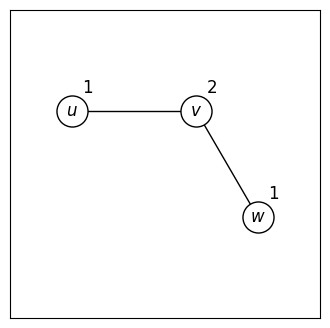
\includegraphics[width=\textwidth]{figures/lwl vs wl-ed/G1.png}
            \caption{$G_1$}
        \end{subfigure}
        \begin{subfigure}[b]{0.25\textwidth}
            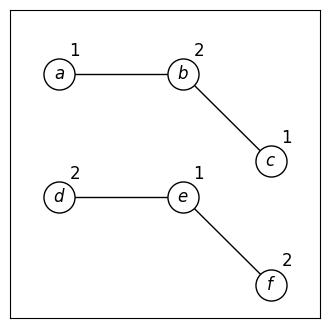
\includegraphics[width=\textwidth]{figures/lwl vs wl-ed/G2.png}
            \caption{$G_2$}
        \end{subfigure}
        \begin{subfigure}[b]{0.25\textwidth}
            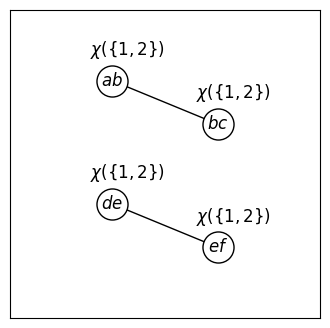
\includegraphics[width=\textwidth]{figures/lwl vs wl-ed/L(G1)-L(G2).png}
            \caption{$L(G_1)=L(G_2)$}
        \end{subfigure}
        \caption{Example of graphs $G_1$, $G_2$ that can be distinguished by $\wledge$ but not by $\lwl$.}
        \label{fig:lwl-wledge-counterexample}
    \end{figure}

    Consider the graphs $G_1$ and $G_2$ depicted in Figure \ref{fig:lwl-wledge-counterexample}.
    $\wledge$ can distinguish between these graphs. To see this, note that the colour $\wl\iter{1}(G_2)(e)$ does not occur anywhere in $\wl\iter{1}(G_1)$, so clearly $\wledge\iter{1}(G_2)(de) \notin \set{\wledge\iter{1}(G_1)(uv) \mid uv\in V(L(G_1))}$.
    In contast, $\lwl$ can never distinguish between $G_1$ and $G_2$, as their line graphs are identical. We conclude that $\lwl$ is strictly less expressive than $\wledge$.
\end{proof}


\section{Proof of Theorem \ref{thm:wledge-equal-to-wl}}   \label{app:proof-wledge-equal-to-wl}

% TODO: say something about injectivity, inverses and the computability thereof


\begin{lemma}   \label{lemma:wl-determines-wledge}
    For any graph $G$, $\multiset{\wl\iter{t+1}(u) \mid u\in G}$ uniquely determines $\multiset{\wledge\iter{t}(uv) \mid uv\in L(G)}$.
\end{lemma}
\begin{proof}
    Due to the injectivity of $\hash$,
    $\multiset{\wl\iter{t+1}(u) \mid u\in G}$
    uniquely determines
    $\multiset{\left(
        \wl\iter{t}(u),
        \multiset{\wl\iter{t}(v) \mid v\in \nbh(u)}
    \right) \mid u\in G}$.

    By iterating over $u\in V(G), v\in\nbh(u)$ and collecting the sets $\set{\wl\iter{t}(u), \wl\iter{t}(v)}$, one uniquely obtains $\multiset{\set{\wl\iter{t}(u), \wl\iter{t}(v)} \mid u\in G, v\in\nbh(u)}$.
    On the other hand, note that the previous iteration goes over every edge exactly twice. Undoubling the elements yields $\multiset{\set{\wl\iter{t}(u), \wl\iter{t}(v)} \mid (u,v)\in E(G)}$, which in turn uniquely determines $\multiset{\wledge\iter{t}(uv) \mid uv\in L(G)}$.

\end{proof}

\begin{lemma}   \label{lemma:wledge-determines-wl}
    $\multiset{\wledge\iter{t}(G_i)(uv) \mid uv\in L(G_i)}$ uniquely determines $\multiset{\wl\iter{t}(u) \mid u\in G_i}$
\end{lemma}
\begin{proof}
    Due to the injectivity of $\dec$,
    $\multiset{\wledge\iter{t}(uv) \mid uv\in L(G_i)}$
    uniquely determines
    $\multiset{\set{\wl\iter{t}(u), \wl\iter{t}(v)} \mid (u,v)\in E(G_i)}$.

    When `unrolling' this multiset -- i.e. creating a multiset that contains both $x$ and $y$ for each $\set{x,y}$ in the original multiset -- we deterministically obtain the multiset that contains $\wl\iter{t}(u)$ exactly $\deg(u)$ times for each $u\in V(G_i)$.

    By the injectivity of $\hash$ and the fact $t>0$, $\wl\iter{t}(u)$ uniquely determines $\deg(u) = \lvert\multiset{\wl\iter{t-1}(v) \mid v\in \nbh(u)}\rvert$ for each $u\in V(G_i)$. So, if we divide the number of occurences of $\wl\iter{t}(u)$ in the unrolled multiset by $\deg(u)$ for each $u$, we deterministically obtain $\multiset{\wl\iter{t}(u) \mid u\in V(G_i)}$.
\end{proof}


\begingroup
\def\thetheorem{\ref{thm:wledge-equal-to-wl}}
\begin{theorem}[restated]
    The $\wledge$-test is equally expressive as the standard WL-test.
\end{theorem}
\addtocounter{theorem}{-1}
\endgroup

\begin{proof}
    Suppose that $\wl$ cannot distinguish between $G_1$ and $G_2$, which implies $\multiset{\wl\iter{t+1}(u) \mid u\in G_1} = \multiset{\wl\iter{t+1}(u) \mid u\in G_2}$ for each $t$.
    Then it follows from lemma \ref{lemma:wl-determines-wledge} that $\multiset{\wledge\iter{t}(uv) \mid uv\in L(G_1) = \multiset{\wledge\iter{t}(uv) \mid uv\in L(G_2)}}$ as well, and hence that $\wledge$ cannot distinguish between $G_1$ and $G_2$ either.

    Similarly, suppose that $\wledge$ cannot distinguish between $G_1$ and $G_2$, which implies $\multiset{\wledge\iter{t}(uv) \mid uv\in L(G_1)} = \multiset{\wledge\iter{t}(uv) \mid uv\in L(G_2)}$ for each $t>0$.
    Then it follows from lemma \ref{lemma:wledge-determines-wl} that $\multiset{\wl\iter{t}(u) \mid u\in G_1} = \multiset{\wl\iter{t}(u) \mid u\in G_2}$ as well for each $t>0$, and hence that $\wl$ cannot distinguish between $G_1$ and $G_2$ either.
\end{proof}


% \begin{equation}
%     \begin{split}
%         &\multiset{\wl\iter{t+1}(u) \mid u\in G_1} = \multiset{\wl\iter{t+1}(u) \mid u\in G_2}
%         \\
%         &\Rightarrow
%         \begin{split}
%             \multiset{\left(
%                 \wl\iter{t}(u),
%                 \multiset{\wl\iter{t}(v) \mid v\in \nbh(u)}
%             \right)}_{u\in G_1}
%             =
%             \multiset{\left(
%                 \wl\iter{t}(u),
%                 \multiset{\wl\iter{t}(v) \mid v\in \nbh(u)}
%             \right)}_{u\in G_2}
%         \end{split}
%     \end{split}
% \end{equation}
% When iterating over all pairs $(u,v)$ with $u\in V(G_i), v\in\nbh(u)$ and collecting the sets $\set{\wl\iter{t}(u), \wl\iter{t}(v)}$ in a multiset, the previous equation implies that the result will be the same for $i\in\set{1,2}$:
% \begin{equation}
%     \multiset{\set{\wl\iter{t}(u), \wl\iter{t}(v)} \mid u\in V(G_1), v\in \nbh(u)} = \multiset{\set{\wl\iter{t}(u), \wl\iter{t}(v)} \mid u\in V(G_2), v\in \nbh(u)}
% \end{equation}
% On the other hand, note that the previously described iteration goes over every edge $(u,v)\in E(G_i)$ exactly twice, so the multisets in the previous equation contain $\set{\wl\iter{t}(u), \wl\iter{t}(v)}$ twice for each edge $(u,v)\in E(G_i)$. Undoubling the elements yields:
% \begin{equation}
%     \begin{split}
%         &\multiset{\set{\wl\iter{t}(u), \wl\iter{t}(v)} \mid (u,v)\in E(G_1)}
%         =
%         \multiset{\set{\wl\iter{t}(u), \wl\iter{t}(v)} \mid (u,v)\in E(G_2)}
%         \\
%         &\Rightarrow
%         \multiset{\wledge\iter{t}(uv) \mid uv\in L(G_1)}
%         =
%         \multiset{\wledge\iter{t}(uv) \mid uv\in L(G_2)}
%     \end{split}
% \end{equation}
% From which follows that $\wledge$ cannot distinguish $G_1$ and $G_2$ either. We conclude that $\wledge$ is at most as expressive as $\wl$.


\bibliographystyle{unsrt}
\bibliography{refs}


\end{document}